\documentclass[12pt, fullpage,letterpaper]{article}

\usepackage[margin=1in]{geometry}
\usepackage{url}
\usepackage{amsmath}
\usepackage{amssymb}
\usepackage{xspace}
\usepackage{graphicx}
\usepackage{hyperref}
\usepackage{listings}

\newcommand{\semester}{Fall 2021}
\newcommand{\assignmentId}{2}
\newcommand{\releaseDate}{28 Sep, 2021}
\newcommand{\dueDate}{11:59pm, 19 Oct, 2021}

\newcommand{\bx}{{\bf x}}
\newcommand{\bw}{{\bf w}}

\title{CS 5350/6350: Machine Learining \semester}
\author{Homework \assignmentId}
\date{Handed out: \releaseDate\\
	Due: \dueDate}


\title{CS 5350/6350: Machine Learning \semester}
\author{Homework \assignmentId}
\date{Handed out: \releaseDate\\
  Due date: \dueDate}

\begin{document}
\maketitle

% Math commands by Thomas Minka
\newcommand{\var}{{\rm var}}
\newcommand{\Tr}{^{\rm T}}
\newcommand{\vtrans}[2]{{#1}^{(#2)}}
\newcommand{\kron}{\otimes}
\newcommand{\schur}[2]{({#1} | {#2})}
\newcommand{\schurdet}[2]{\left| ({#1} | {#2}) \right|}
\newcommand{\had}{\circ}
\newcommand{\diag}{{\rm diag}}
\newcommand{\invdiag}{\diag^{-1}}
\newcommand{\rank}{{\rm rank}}
% careful: ``null'' is already a latex command
\newcommand{\nullsp}{{\rm null}}
\newcommand{\tr}{{\rm tr}}
\renewcommand{\vec}{{\rm vec}}
\newcommand{\vech}{{\rm vech}}
\renewcommand{\det}[1]{\left| #1 \right|}
\newcommand{\pdet}[1]{\left| #1 \right|_{+}}
\newcommand{\pinv}[1]{#1^{+}}
\newcommand{\erf}{{\rm erf}}
\newcommand{\hypergeom}[2]{{}_{#1}F_{#2}}

% boldface characters
\renewcommand{\a}{{\bf a}}
\renewcommand{\b}{{\bf b}}
\renewcommand{\c}{{\bf c}}
\renewcommand{\d}{{\rm d}}  % for derivatives
\newcommand{\e}{{\bf e}}
\newcommand{\f}{{\bf f}}
\newcommand{\g}{{\bf g}}
\newcommand{\h}{{\bf h}}
%\newcommand{\k}{{\bf k}}
% in Latex2e this must be renewcommand
\renewcommand{\k}{{\bf k}}
\newcommand{\m}{{\bf m}}
\newcommand{\mb}{{\bf m}}
\newcommand{\n}{{\bf n}}
\renewcommand{\o}{{\bf o}}
\newcommand{\p}{{\bf p}}
\newcommand{\q}{{\bf q}}
\renewcommand{\r}{{\bf r}}
\newcommand{\s}{{\bf s}}
\renewcommand{\t}{{\bf t}}
\renewcommand{\u}{{\bf u}}
\renewcommand{\v}{{\bf v}}
\newcommand{\w}{{\bf w}}
\newcommand{\x}{{\bf x}}
\newcommand{\y}{{\bf y}}
\newcommand{\z}{{\bf z}}
%s\newcommand{\l}{\boldsymbol{l}}
\newcommand{\A}{{\bf A}}
\newcommand{\B}{{\bf B}}
\newcommand{\C}{{\bf C}}
\newcommand{\D}{{\bf D}}
\newcommand{\E}{{\bf E}}
\newcommand{\F}{{\bf F}}
\newcommand{\G}{{\bf G}}
\renewcommand{\H}{{\bf H}}
\newcommand{\I}{{\bf I}}
\newcommand{\J}{{\bf J}}
\newcommand{\K}{{\bf K}}
\renewcommand{\L}{{\bf L}}
\newcommand{\M}{{\bf M}}
\newcommand{\N}{\mathcal{N}}  % for normal density
%\newcommand{\N}{{\bf N}}
\renewcommand{\O}{{\bf O}}
\renewcommand{\P}{{\bf P}}
\newcommand{\Q}{{\bf Q}}
\newcommand{\R}{{\bf R}}
\renewcommand{\S}{{\bf S}}
\newcommand{\T}{{\bf T}}
\newcommand{\U}{{\bf U}}
\newcommand{\V}{{\bf V}}
\newcommand{\W}{{\bf W}}
\newcommand{\X}{{\bf X}}
\newcommand{\Y}{{\bf Y}}
\newcommand{\Z}{{\bf Z}}

% this is for latex 2.09
% unfortunately, the result is slanted - use Latex2e instead
%\newcommand{\bfLambda}{\mbox{\boldmath$\Lambda$}}
% this is for Latex2e
\newcommand{\bfLambda}{\boldsymbol{\Lambda}}

% Yuan Qi's boldsymbol
\newcommand{\bsigma}{\boldsymbol{\sigma}}
\newcommand{\balpha}{\boldsymbol{\alpha}}
\newcommand{\bpsi}{\boldsymbol{\psi}}
\newcommand{\bphi}{\boldsymbol{\phi}}
\newcommand{\boldeta}{\boldsymbol{\eta}}
\newcommand{\Beta}{\boldsymbol{\eta}}
\newcommand{\btau}{\boldsymbol{\tau}}
\newcommand{\bvarphi}{\boldsymbol{\varphi}}
\newcommand{\bzeta}{\boldsymbol{\zeta}}

\newcommand{\blambda}{\boldsymbol{\lambda}}
\newcommand{\bLambda}{\mathbf{\Lambda}}
\newcommand{\bOmega}{\mathbf{\Omega}}
\newcommand{\bomega}{\mathbf{\omega}}
\newcommand{\bPi}{\mathbf{\Pi}}

\newcommand{\btheta}{\boldsymbol{\theta}}
\newcommand{\bpi}{\boldsymbol{\pi}}
\newcommand{\bxi}{\boldsymbol{\xi}}
\newcommand{\bSigma}{\boldsymbol{\Sigma}}

\newcommand{\bgamma}{\boldsymbol{\gamma}}
\newcommand{\bGamma}{\mathbf{\Gamma}}

\newcommand{\bmu}{\boldsymbol{\mu}}
\newcommand{\1}{{\bf 1}}
\newcommand{\0}{{\bf 0}}

% \newcommand{\comment}[1]{}

\newcommand{\bs}{\backslash}
\newcommand{\ben}{\begin{enumerate}}
\newcommand{\een}{\end{enumerate}}

 \newcommand{\notS}{{\backslash S}}
 \newcommand{\nots}{{\backslash s}}
 \newcommand{\noti}{{\backslash i}}
 \newcommand{\notj}{{\backslash j}}
 \newcommand{\nott}{\backslash t}
 \newcommand{\notone}{{\backslash 1}}
 \newcommand{\nottp}{\backslash t+1}
% \newcommand{\notz}{\backslash z}

\newcommand{\notk}{{^{\backslash k}}}
%\newcommand{\noti}{{^{\backslash i}}}
\newcommand{\notij}{{^{\backslash i,j}}}
\newcommand{\notg}{{^{\backslash g}}}
\newcommand{\wnoti}{{_{\w}^{\backslash i}}}
\newcommand{\wnotg}{{_{\w}^{\backslash g}}}
\newcommand{\vnotij}{{_{\v}^{\backslash i,j}}}
\newcommand{\vnotg}{{_{\v}^{\backslash g}}}
\newcommand{\half}{\frac{1}{2}}
\newcommand{\msgb}{m_{t \leftarrow t+1}}
\newcommand{\msgf}{m_{t \rightarrow t+1}}
\newcommand{\msgfp}{m_{t-1 \rightarrow t}}

\newcommand{\proj}[1]{{\rm proj}\negmedspace\left[#1\right]}
\newcommand{\argmin}{\operatornamewithlimits{argmin}}
\newcommand{\argmax}{\operatornamewithlimits{argmax}}

\newcommand{\dif}{\mathrm{d}}
\newcommand{\abs}[1]{\lvert#1\rvert}
\newcommand{\norm}[1]{\lVert#1\rVert}

%miscellaneous symbols
\newcommand{\ie}{{{i.e.,}}\xspace}
\newcommand{\eg}{{{\em e.g.,}}\xspace}
\newcommand{\EE}{\mathbb{E}}
\newcommand{\VV}{\mathbb{V}}
\newcommand{\sbr}[1]{\left[#1\right]}
\newcommand{\rbr}[1]{\left(#1\right)}
\newcommand{\cmt}[1]{}



\section{Paper Problems [40 points + 8 bonus]}
\begin{enumerate}
\item~
\[
m > \frac{1}{\epsilon}\big(\log(|H|) + \log\frac{1}{\delta}\big).
\]

\begin{enumerate}
	\item~
	\begin{enumerate}
		\item~\emph{Answer}
		
		We desire an answer that requires the least amount of data with some minimum level of confidence.
		
		\item~\emph{Answer}
		
		This principle is reflected in the $log|H|$ term which is monotonic increasing for $|H|>0$, so smaller $|H|$ implies a smaller number of necessary examples $m$.
		
	\end{enumerate}
	\item~\emph{Answer}
	
	\[
        |H| = 3^{n}, n=10 => |H|=3^{10}=59,049
	\]
	\[
	    \epsilon=1-0.9=0.1, 1-\delta=0.95 => \delta=0.05
	\]
	\[
	    => m>\frac{1}{0.1}*(log|59,049|+log\frac{1}{0.05})
	\]
	\[
	    m>139.8
	\]
	
	Therefore, we require at least 140 training examples.
	
\end{enumerate}

\item~\emph{Answer}

First, note that when $y_i = h_t(x_i)$ then $y_i * h_t(x_i) = 1$, and conversely when $y_i \neq h_t(x_i)$ then $y_i * h_t(x_i) = -1$.

\[
    => \epsilon_t = \frac{1}{2} - \frac{1}{2}\big(\sum_{y_i = h_t(x_i)} D_t(i) - \sum_{y_i \neq h_t(x_i)} D_t(i)\big)
\]

We then note that $\sum_{i=1}^m D_t(i) = 1$, which can be split into: 

\[\sum_{y_i = h_t(x_i)} D_t(i) + \sum_{y_i \neq h_t(x_i)} D_t(i)=1\]

\[
    => \epsilon_t = \frac{1}{2}\big(\sum_{y_i = h_t(x_i)} D_t(i) + \sum_{y_i \neq h_t(x_i)} D_t(i)\big) - \frac{1}{2}\big(\sum_{y_i = h_t(x_i)} D_t(i) - \sum_{y_i \neq h_t(x_i)} D_t(i)\big)
\]

\[
    = \frac{1}{2}\sum_{y_i = h_t(x_i)} D_t(i) + \frac{1}{2}\sum_{y_i \neq h_t(x_i)} D_t(i) - \frac{1}{2}\sum_{y_i = h_t(x_i)} D_t(i) + \frac{1}{2}\sum_{y_i \neq h_t(x_i)} D_t(i)
\]

\[
    = \sum_{y_i \neq h_t(x_i)} D_t(i)_\blacksquare
\]

\item~
	\begin{enumerate}
		\item~[2 point] $f(x_1, x_2, x_3) = x_1 \land \neg x_2 \land \neg x_3$
		
		\emph{Answer}
		
		Based on that logic function, would expect $y=1$ if $x_1-x_2-x_3>=1$. Table 1 results prove that this function works, so the hyperplane is $y=x_1-x_2-x_3-1$, $bias=-1$, and the weight vector is $[1, -1, -1]$.
		
		\begin{table}
        	\centering
        	\begin{tabular}{ccccc|c}
        		$x_1 $ & $x_2$ & $x_3$ & $y$ & $x_1-x_2-x_3-1$ & $sign$\\ 
        		\hline\hline
        		0 & 0 & 0 & 0 & -1 & 0 \\ \hline
        		0 & 0 & 1 & 0 & -2 & 0 \\ \hline
        		0 & 1 & 0 & 0 & -2 & 0 \\ \hline
        		0 & 1 & 1 & 0 & -3 & 0 \\ \hline
        		1 & 0 & 0 & 1 &  0 & 1 \\ \hline
        		1 & 0 & 1 & 0 & -1 & 0 \\ \hline
        		1 & 1 & 0 & 0 & -1 & 0 \\ \hline
        		1 & 1 & 1 & 0 & -2 & 0 \\ \hline
        	\end{tabular}
        	\caption{Table of answers for 3a.}\label{tb:1}
        \end{table}
		
		\item~[2 point] $f(x_1, x_2, x_3) = \neg x_1 \lor \neg x_2 \lor \neg x_3$ 
		
		\emph{Answer}
		
		Based on that logic function, would expect $y=1$ if $x_1+x_2+x_3<=-2$. Table 2 results prove that this function works, so the hyperplane is $y=2-x_1-x_2-x_3$, $bias=2$, and the weight vector is $[-1, -1, -1]$.
		
		\begin{table}
        	\centering
        	\begin{tabular}{ccccc|c}
        		$x_1 $ & $x_2$ & $x_3$ & $y$ & $2-x_1-x_2-x_3$ & $sign$\\ 
        		\hline\hline
        		0 & 0 & 0 & 1 &  2 & 1 \\ \hline
        		0 & 0 & 1 & 1 &  1 & 1 \\ \hline
        		0 & 1 & 0 & 1 &  1 & 1 \\ \hline
        		0 & 1 & 1 & 1 &  0 & 1 \\ \hline
        		1 & 0 & 0 & 1 &  1 & 1 \\ \hline
        		1 & 0 & 1 & 1 &  0 & 1 \\ \hline
        		1 & 1 & 0 & 1 &  0 & 1 \\ \hline
        		1 & 1 & 1 & 0 & -1 & 0 \\ \hline
        	\end{tabular}
        	\caption{Table of answers for 3b.}\label{tb:1}
        \end{table}
		
		\item~[8 points] $f(x_1, x_2, x_3, x_4) = (x_1 \lor x_2) \land (x_3 \lor x_4)$
		
		\emph{Answer}
		
		Based on that logic function, would expect $y=1$ if $(x_1+x_2)+(x_3+x_4)>=2$, but this doesn't work because if $x_1=x_2=1$ and $x_3=x_4=0$ then $y=1$ instead of $0$. Instead, let's try a feature mapping that multiplies items in each logic parenthetical together, which yields $(x_1+x_2-x_1x_2)+(x_3+x_4-x_3x_4)>=2$. Table 3 results prove that this function works, so the hyperplane is $y=(x_1+x_2-x_1x_2)+(x_3+x_4-x_3x_4)-2=x_1(1-x_2)+x_2+x_3(1-x_4)+x_4-2$. The $bias=-2$, and the weight vector is $[1-x_2, 1, 1-x_4, 1]$.
		
		\begin{table}
        	\centering
        	\begin{tabular}{cccccc|c}
        		$x_1 $ & $x_2$ & $x_3$ & $x_4$ & $y$ & $2-x_1-x_2-x_3$ & $sign$\\ 
        		\hline\hline
        		0 & 0 & 0 & 0 & 0 & -2 & 0 \\ \hline
        		0 & 0 & 0 & 1 & 0 & -1 & 0 \\ \hline
        		0 & 0 & 1 & 0 & 0 & -1 & 0 \\ \hline
        		0 & 0 & 1 & 1 & 0 & -1 & 0 \\ \hline
        		0 & 1 & 0 & 0 & 0 & -1 & 0 \\ \hline
        		0 & 1 & 0 & 1 & 1 &  0 & 1 \\ \hline
        		0 & 1 & 1 & 0 & 1 &  0 & 1 \\ \hline
        		0 & 1 & 1 & 1 & 1 &  0 & 1 \\ \hline
        		1 & 0 & 0 & 0 & 0 & -1 & 0 \\ \hline
        		1 & 0 & 0 & 1 & 1 &  0 & 1 \\ \hline
        		1 & 0 & 1 & 0 & 1 &  0 & 1 \\ \hline
        		1 & 0 & 1 & 1 & 1 &  0 & 1 \\ \hline
        		1 & 1 & 0 & 0 & 0 & -1 & 0 \\ \hline
        		1 & 1 & 0 & 1 & 1 &  0 & 1 \\ \hline
        		1 & 1 & 1 & 0 & 1 &  0 & 1 \\ \hline
        		1 & 1 & 1 & 1 & 1 &  0 & 1 \\ \hline
        	\end{tabular}
        	\caption{Table of answers for 3c.}\label{tb:1}
        \end{table}
        
		\item ~[8 points] $f(x_1, x_2) = (x_1 \land x_2) \lor (\neg x_1 \land \neg x_2)$
		
		\emph{Answer}
		
		Based on that logic function, would expect $y=1$ if $(x_1+x_2-2)+(-x_1-x_2)>=1$, but this doesn't work because $x_1$ and $x_2$ cancel out, yielding $-3>=1$, which is false. Instead, let's try a feature mapping that squares each parenthetical, yielding $(x_1+x_2-2)^2+(-x_1-x_2)^2>=1$. But this doesn't work when $x_1=0, x_2=1$ because that yields a true statement when it \emph{should} be false. I note that when $x_1=x_2=1$, then $y=3$, so, what if we just up the bias from $-1$ to $-3$ so when $x_1=x_2=1$ would yield $y=1$. Table 4 results prove that this function works, so the hyperplane is $y=(x_1+x_2-2)^2+(-x_1-x_2)^2-3$, which if we expand it becomes $y=2x_1^2+2x_2^2+4x_1x_2-4x_1-4x_2=x_1(2x_1+4x_2-4)+x_2(2x_2-4)$. The $bias=0$, with a weight vector of $[2x_1+4x_2-4, 2x_2-4]$.
		
		\begin{table}
        	\centering
        	\begin{tabular}{cccc|c}
        		$x_1 $ & $x_2$ & $y$ & $(x_1+x_2-2)^2+(-x_1-x_2)^2-3$ & $sign$\\ 
        		\hline\hline
        		0 & 0 & 1 &  0 & 1 \\ \hline
        		0 & 1 & 0 & -2 & 0 \\ \hline
        		1 & 0 & 0 & -2 & 0 \\ \hline
        		1 & 1 & 1 &  0 & 1 \\ \hline
        	\end{tabular}
        	\caption{Table of answers for 3d.}\label{tb:1}
        \end{table}
	\end{enumerate}
		
	
	\item~
	\begin{enumerate}
		\item~\emph{Answer}
		
		\[
		    (\x^\top \y)^2 = x_1^2y_1^2 + 2x_1y_1x_2y_2 + x_2^2y_2^2
		\]
		\[
            => \phi(\x) = x_1^2\hat{i} + \sqrt{2}x_1x_2\hat{j} + x_2^2\hat{k}
        \]
		\[
            => \phi(\y) = y_1^2\hat{i} + \sqrt{2}y_1y_2\hat{j} + y_2^2\hat{k}
        \]
        
        
		
		\item~\emph{Answer}
		
		\[
		    (\x^\top \y)^3 = x_1^3y_1^3 + 3x_1^2y_1^2x_2y_2 + 3x_1y_1x_2^2y_2^2 + x_2^3y_2^3
		\]
		\[
            => \phi(\x) = x_1^3\hat{i} + \sqrt{3}x_1^2x_2\hat{j} + \sqrt{3}x_1x_2^2\hat{k} + x_2^3\hat{l}
        \]
		\[
            => \phi(\y) = y_1^3\hat{i} + \sqrt{3}y_1^2y_2\hat{j} + \sqrt{3}y_1y_2^2\hat{k} + y_2^3\hat{l}
        \]
        
		\item~\emph{Answer}
		
		Seems to possibly correspond to the Binomial Theorem, $(x+y)^n = \sum_{k=0}^n {n \choose k}x^{n-k}y^k$. However, the difference here would be that for $\phi(\a)$ the $n \choose k$ term becomes $\sqrt{n \choose k}$. Will check a few more to be sure.
		
		\[
		    (\x^\top \y)^4 = x_1^4y_1^4 + 4x_1^3y_1^3x_2y_2 + 6x_1^2y_1^2x_2^2y_2^2 + 4x_1y_1x_2^3y_2^3 + x_2^4y_2^4
		\]
		\[
            => \phi(\x) = x_1^4\hat{i} + \sqrt{4}x_1^3x_2\hat{j} + \sqrt{6}x_1^2x_2^2\hat{k} + \sqrt{4}x_1x_2^3\hat{l} + x_2^4\hat{m}
        \]
		\[
            => \phi(\y) = y_1^4\hat{i} + \sqrt{4}y_1^3y_2\hat{j} + \sqrt{6}y_1^2y_2^2\hat{k} + \sqrt{4}y_1y_2^3\hat{l} + y_2^4\hat{m}
        \]
        
        \[
		    (\x^\top \y)^5 = x_1^5y_1^5 + 5x_1^4y_1^4x_2y_2 + 10x_1^3y_1^3x_2^2y_2^2 + 10x_1^2y_1^2x_2^3y_2^3 + 5x_1y_1x_2^4y_2^4 + x_2^5y_2^5
		\]
		\[
            => \phi(\x) = x_1^5\hat{i} + \sqrt{5}x_1^4x_2\hat{j} + \sqrt{10}x_1^3x_2^2\hat{k} + \sqrt{10}x_1^2x_2^3\hat{l} + \sqrt{5}x_1x_2^4\hat{m} + x_2^5\hat{n}
        \]
		\[
            => \phi(\y) = y_1^5\hat{i} + \sqrt{5}y_1^4y_2\hat{j} + \sqrt{10}y_1^3y_2^2\hat{k} + \sqrt{10}y_1^2y_2^3\hat{l} + \sqrt{5}y_1y_2^4\hat{m} + y_2^5\hat{n}
        \]
        
        By induction, we can apply the Binomial Theorem to $(\x^\top \y)^k$ with the changes described above. This leads to:
        
        \[
            \phi(\x) = \sum_{i=0}^k \sqrt{k \choose i} x_1^{k-i} x_2^{i} \hat{i}
        \]
        \[
            \phi(\y) = \sum_{i=0}^k \sqrt{k \choose i} y_1^{k-i} y_2^{i} \hat{i}
        \]
		
	\end{enumerate}

\item~  
\begin{table}
	\centering
	\begin{tabular}{ccc|c}
		$x_1 $ & $x_2$ & $x_3$ &  $y$\\ 
		\hline\hline
		1 & -1 & 2 & 1 \\ \hline
		1 & 1 & 3 & 4 \\ \hline
		-1 & 1 & 0 & -1 \\ \hline
		1 & 2 & -4 & -2 \\ \hline
		3 & -1 & -1 & 0\\ \hline
	\end{tabular}
	\caption{Linear regression training data.}\label{tb:1}
\end{table}

\begin{enumerate}
	\item~\emph{Answer}
	
	The bias is baked into the weights term, so we just need to extract it from regular $J(\w)$.
	
	\[
	    J(\w) = \sum_{i=1}^m (y_i - \w^\top \x_i)^2
	\]
	\[
	    => J(\w, b) = \sum_{i=1}^m (y_i - \w^\top \x_i - b)^2
	\]
	
	\item~\emph{Answer}
	
	Code for solution can be found in Listing 1. The function q5b specifically calculates the gradient for the parameters and data (see Table 5) specified. In this case, we find the gradient to be:
	
	\[
	\frac{dJ}{dw_1} = -22
	\]
	\[
    \frac{dJ}{dw_2} = 16
    \]
    \[
    \frac{dJ}{dw_3} = -56
    \]
    \[
    \frac{dJ}{db} = -10
    \]
	
	\begin{lstlisting}[language=Python, caption=QuestionAnswers.part1]

import numpy as np


def q5b():
    x1 = np.array([1, 1, -1, 1, 3])
    x2 = np.array([-1, 1, 1, 2, -1])
    x3 = np.array([2, 3, 0, -4, -1])
    X = np.array([x1, x2, x3]).T
    y = np.array([1, 4, -1, -2, 0]).T
    w = np.array([-1, 1, -1])
    b = -1
    for j in range(len(w)):
        x_j = X[:, j]
        djdw = calc_djdw(X, y, w, b, x_j)
        print(f'dJ_dw_{j + 1}: {djdw}')
    djdb = calc_djdb(X, y, w, b)
    print(f'dJ_db: {djdb}')


def q5c():
    x1 = np.array([1, 1, -1, 1, 3])
    x2 = np.array([-1, 1, 1, 2, -1])
    x3 = np.array([2, 3, 0, -4, -1])
    y = np.array([1, 4, -1, -2, 0]).T
    y_x1 = -np.dot(x1, y)
    print(f'y_x1: {y_x1}')
    y_x2 = -np.dot(x2, y)
    print(f'y_x2: {y_x2}')
    y_x3 = -np.dot(x3, y)
    print(f'y_x3: {y_x3}')
    
    x1_x1 = -np.dot(x1, x1)
    print(f'x1_x1: {x1_x1}')
    x1_x2 = -np.dot(x1, x2)
    print(f'x1_x2: {x1_x2}')
    x1_x3 = -np.dot(x1, x3)
    print(f'x1_x3: {x1_x3}')

    x2_x1 = -np.dot(x2, x1)
    print(f'x2_x1: {x2_x1}')
    x2_x2 = -np.dot(x2, x2)
    print(f'x2_x2: {x2_x2}')
    x2_x3 = -np.dot(x2, x3)
    print(f'x2_x3: {x2_x3}')

    x3_x1 = -np.dot(x3, x1)
    print(f'x3_x1: {x3_x1}')
    x3_x2 = -np.dot(x3, x2)
    print(f'x3_x2: {x3_x2}')
    x3_x3 = -np.dot(x3, x3)
    print(f'x3_x3: {x3_x3}')


def q5d():
    x1 = np.array([1, 1, -1, 1, 3])
    x2 = np.array([-1, 1, 1, 2, -1])
    x3 = np.array([2, 3, 0, -4, -1])
    X = np.array([x1, x2, x3]).T
    y = np.array([1, 4, -1, -2, 0]).T
    w = np.array([0.0, 0.0, 0.0])
    b = 0
    r = 0.1
    for i in range(5):
        for j in range(len(w)):
            djdw = calc_djdw(X[i], y[i], w, b, X[i, j])
            print(f'round {i + 1}, weight updated {j + 1}: {w[j]} + {r * djdw} = {w[j] + r * djdw}')
            w[j] = w[j] + r * djdw
        djdb = calc_djdb(X[i], y[i], w, b)
        print(f'round {i + 1}, bias updated: {b} + {r * djdb} = {b + r * djdb}')
        b = b + r * djdb
    s = 0
    for k in w:
        print(f'w_{s + 1}: {k}')
        s += 1
    print(f'b: {b}')


def calc_djdw(X, y, w, b, x_j):
    return -np.sum(np.dot((y - np.dot(X, w) - b), x_j))


def calc_djdb(X, y, w, b):
    return -np.sum(y - np.dot(X, w) - b)


def calc_cost(X, y, w, b):
    return 0.5 * np.sum(np.square(y - np.dot(X, w) - b))


	\end{lstlisting}
	
	\item~\emph{Answer}
	
	\[
	    J(\w, b) = \frac{1}{2} \sum_{i=1}^m (y_i - \w^\top \x_i - b)^2
	\]
	\[
        => \frac{dJ}{dw_j} = -\sum_{i=1}^m (y_i - \w^\top \x_i - b)x_{ij},  \frac{dJ}{db} = -\sum_{i=1}^m (y_i - \w^\top \x_i - b)
    \]
    Plugging in the data from Table 5, we see that:
    \[
       \frac{dJ}{db} = -2 + 5w_1 +2 w_2 + 0w_3 + 5b
    \]
    Setting this equal to 0 to minimize,
    \[
        => b = \frac{2}{5} - w_1 - \frac{2}{5}w_2
    \]
    \[
        => \frac{dJ}{dw_j} = -\sum_{i=1}^m (y_i x_{ij} - w_1 x_{i1} x_{ij} - w_2 x_{i2} x_{ij} - w_3 x_{i3} x_{ij} - b x_{ij})
    \]
    \[
        = -\sum_{i=1}^m y_i x_{ij} + w_1\sum_{i=1}^m x_{i1} x_{ij} + w_2\sum_{i=1}^m x_{i2} x_{ij} + w_3\sum_{i=1}^m x_{i3} x_{ij} + b\sum_{i=1}^m x_{ij}
    \]
    Function q5c in Listing 1 will calculate the sums above, giving us:
    \[
        \frac{dJ}{dw_1} = 4 - 13w_1 + 2w_2 + 2w_3 - 2 + 5w_1 + 2w_2 = 2 - 8w_1 + 4w_2 + 2w_3 = 0
    \]
    \[
        \frac{dJ}{dw_2} = -2 + 2w_1 - 8w_2 + 6w_3 - \frac{4}{5} + 2w_1 + \frac{4}{5}w_2 = -\frac{14}{5} + 4w_1 - \frac{36}{5}w_2 + 6w_3 = 0
    \]
    \[
        \frac{dJ}{dw_3} = 22 + 2w_1 + 6w_2 - 30w_3 - \frac{4}{5} + 2w_1 + \frac{4}{5}w_2 = -\frac{106}{5} + 4w_1 + \frac{34}{5}w_2 - 30w_3 = 0
    \]
    
    Plugging this system of equations into \href{https://www.wolframalpha.com/input/?i=systems+of+equations+calculator&assumption=%7B%22F%22%2C+%22SolveSystemOf3EquationsCalculator%22%2C+%22equation1%22%7D+-%3E%222-8a%2B4b%2B2c%22&assumption=%22FSelect%22+-%3E+%7B%7B%22SolveSystemOf3EquationsCalculator%22%7D%7D&assumption=%7B%22F%22%2C+%22SolveSystemOf3EquationsCalculator%22%2C+%22equation2%22%7D+-%3E%22-14%2F5%2B4a-36%2F5b%2B6c%22&assumption=%7B%22F%22%2C+%22SolveSystemOf3EquationsCalculator%22%2C+%22equation3%22%7D+-%3E%22106%2F5%2B4a%2B34%2F5b-30c%22}{Wolfram Alpha} (click for link), we get that:
    \[
        w_1 = \frac{247}{223}
    \]
    \[
        w_2 = \frac{258}{223}
    \]
    \[
        w_3 = \frac{249}{223}
    \]
    Which, plugging this back into our equation for $b$, we see that:
    \[
        b = -1.17_\blacksquare
    \]
	
	\item~\emph{Answer}
	
	Function q5d in Listing 1 gives these results:
	
	\emph{Round 1}:
	
	weight updated 1: $0.0 + -0.1 = -0.1$
	
	weight updated 2: $0.0 + 0.1100 = 0.1100$
    
    weight updated 3: $0.0 + -0.242 = -0.242$
    
    bias updated: $0 + -0.1694 = -0.1694$
    
    \emph{Round 2}:
    
    weight updated 1: $-0.1 + -0.4885 = -0.5885$
    
    weight updated 2: $0.1100 + -0.5374 = -0.4274$
    
    weight updated 3: $-0.2420 + -1.7734 = -2.0154$
    
    bias updated: $-0.1694 + -1.1232 = -1.2926$
    
    \emph{Round 3}:
    
    weight updated 1: $-0.5885 + 0.0131 = -0.5754$
    
    weight updated 2: $-0.4274 + -0.0145 = -0.4418$
    
    weight updated 3: $-2.0154 + -0.0 = -2.0154$
    
    bias updated: $-1.2926 + -0.0159 = -1.3085$
    
    \emph{Round 4}:
    
    weight updated 1: $-0.5754 + 0.7294 = 0.1540$
    
    weight updated 2: $-0.4418 + 1.6047 = 1.1628$
    
    weight updated 3: $-2.0154 + -4.4931 = -6.5085$
    
    bias updated: $-1.3085 + 2.9205 = 1.6121$
    
    \emph{Round 5}:
    
    weight updated 1: $0.1540 + 2.2259 = 2.3799$
    
    weight updated 2: $1.1628 + -1.4098 = -0.2469$
    
    weight updated 3: $-6.5085 + -1.5507 = -8.0593$
    
    bias updated: $1.6121 + 1.7058 = 3.3179$
    
    \emph{Final Results}
    
    $w_1 = 2.3799$
    
    $w_2 = -0.2469$
    
    $w_3 = -8.0593$
    
    $b = 3.3179$
	
\end{enumerate}
\end{enumerate}

\section{Practice [60 points + 10 bonus]}
\begin{enumerate}
	\item~\emph{Answer}
	
	\href{https://github.com/Paul-Wissler/cs-6350-hw2}{Click here for the repository for HW2}. It is not the same as the repository for HW1.

\item~
\begin{enumerate}
	\item~\emph{Answer}
	
	Figure 1 shows how Adaboost performs, while Figure 2 shows how individual tree stumps perform. Obviously, this shows that Adaboost performs better, converging to some final error after ~100 rounds, while the individual tree stumps continue to oscillate between 20\% and 80\% error. Comparing Figure 1 to HW1 Table 10 (data used to generate test results for q3a), which shows the accuracy of the data, we can infer that Adaboost performs a bit better on Test data, coming to about 10.7\% error rate, while the best performing tree in Table 10 had an error rate of about 11.3\%. More importantly, though, is that Adaboost seems to be better at reliably generating a well-performing tree with more iterations, making it more stable, while the results in HW1 Table 10 clearly show that the results got \emph{worse} with deeper trees due to over-fitting. I.e., Adaboost's primary advantage over a single tree is that it seems less prone to over-fitting, making it a more reliable model.
	
	\begin{figure}[htp]
        \centering
        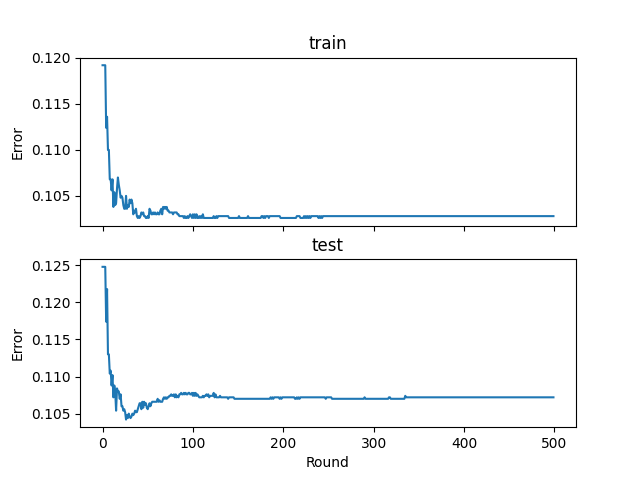
\includegraphics[width=12cm]{q2a_cum_results.png}
        \caption{Training and Test Errors for q2a, Adaboost algorithm after T rounds.}
        \label{fig:q4a}
    \end{figure}
    
    \begin{figure}[htp]
        \centering
        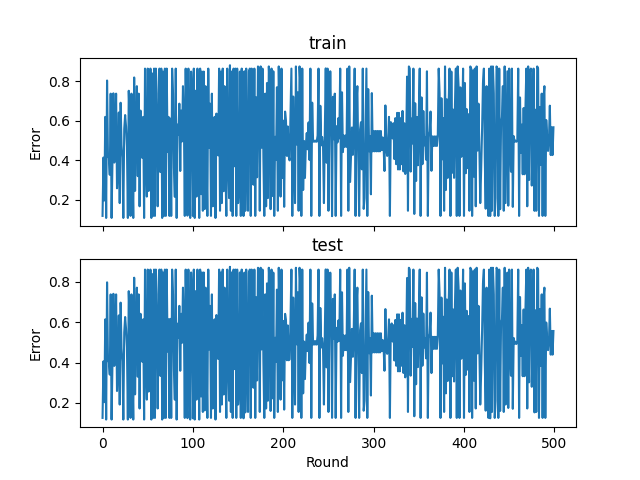
\includegraphics[width=12cm]{q2a_single_results.png}
        \caption{Training and Test Errors for q2a, individual trees over rounds.}
        \label{fig:q4a}
    \end{figure}
	
	\item~\emph{Answer}
	
	The results for this question can be found in Figure 3. Based merely on these results, I would say that Adaboost performs better than Bagging, as Adaboost converged to around 10.7\% error on the test data, while bagging converged to around 11.9\%. Interestingly, Adaboost actually had similar performance on both the training and test data, which would indicate that it is less sensitive to over-fitting, while bagging performs better on training data, similar to what we saw with individual trees. The errors still converge, though, making bagging better than single trees. 
	
	Another interesting note is that the test error was lower on a small number of trees, similar to how a single decision tree with a relatively shallow depth performs better on test data than their full-depth counterparts, though this may simply be a coincidence
	
	\begin{figure}[htp]
        \centering
        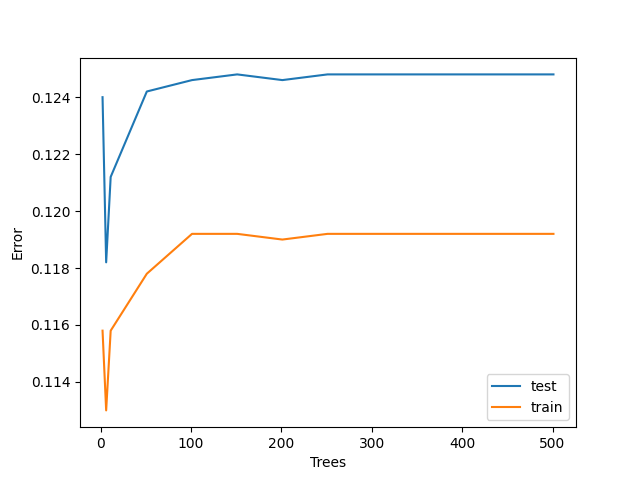
\includegraphics[width=12cm]{q2b_plot.png}
        \caption{Training and Test Errors for q2b.}
        \label{fig:q4a}
    \end{figure}

	\item~\emph{Answer}
	
	RESULTS:
	
	Single Tree Bias: 0.1060

    Single Tree Sample Variance: 0.0462
    
    Single Tree General Squared Error: 0.1395
    
    Bagged Trees Bias: 0.1246864
    
    Bagged Trees Sample Variance: 0.0001
    
    Bagged Trees General Squared Error: 0.1248
    
    From these results, it seems that the general squared error for Bagged Trees is a bit better than Single Trees. However, Bagged Trees are considerably more biased, but with much smaller variance. From this, I would conclude that Bagged Trees are a more reliable way to make models than single trees. I would be curious to see how limiting tree depth changes Bagged Trees General Squared Error. Based on what I have seen with full-depth trees in HW1, I would expect the General Squared Error to decrease.
	 
	\item~\emph{Answer}
	
	Figure 4 shows how well the Random Forest performed. Based merely on these results, I would say that bagging performs better, likely because it has more data to work with when creating its trees, while Random Forests limit themselves to a small number of attributes. To be specific, on test data, bagging error converged to around 12.5\% error, while Random Forests with 4 and 6 attributes sampled converged to around 13\% error. However, this is not a massive difference, and the error for Random Forests that sample 2 attributes was about 12.5\% as well. There is also the performance to consider, as Random Forests run faster than full bagging based on experience (but with no data to support this claim). 
	
	I take these results with a grain of salt, however, as based on the results seen in q2e, I think that what is happening is that the Random Forest ends up simply taking the mode of the dependent values in training, and assumes all inputs map to that one output. This is most likely a bug with my implementation, but I do not know how to properly fix it. This is also reinforced by how there is almost no convergence curve for all results in Figure 4, especially for when only 2 attributes are sampled, as that is just a straight line for both training and test results.
	
	\begin{figure}[htp]
        \centering
        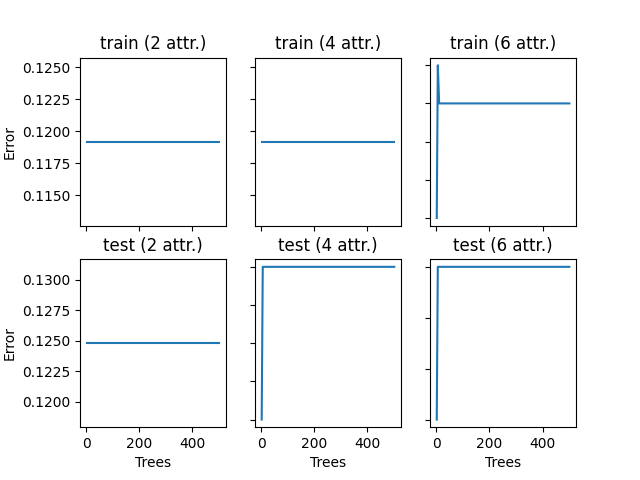
\includegraphics[width=12cm]{q2d_plot.png}
        \caption{Training and Test Errors for q2d, random forest sampling 2, 4, or 6 attributes.}
        \label{fig:q4a}
    \end{figure}
	
	\item~\emph{Answer}
	
	Single Tree Bias: 0.11706194
	
    Single Tree Sample Variance: 0.021604101010101014
    
    Single Tree General Squared Error: 0.13106269212272728
    
    Full Forest Bias: 0.1248
    
    Full Forest Sample Variance: 0.0
    
    Full Forest General Squared Error: 0.1248
    
    As we saw in q2c with Bagged Trees, the Full Forest has a smaller error than Single Trees due to a much smaller variance, but with a higher bias. In this case, however, I do not trust these results as indicated in my answer to q2d. The reason why can be seen in the sample variance for the Full Forest, which is exactly 0. On checking the output results from my Random Forest algorithm, I saw that it predicted the same results every single time, and that result was the mode of the training output values. So, it would seem that my Random Forest ends up predicting the mode for any given input. Based on these results, I conclude that there is likely a bug in my implementation. It is possible that tuning my parameters will yield better results. However, taking these results as truth, I would conclude that Bagged Trees and Random Forests tend to be highly biased but with very low variance, making them more reliable than Single Trees overall.
    
	
\end{enumerate}

\item~\emph{Answer}

Figures 5-8 show how Decision Trees, Adaboost, Bagged Trees, and Random Forests respectively dealt with the credit default data. Figures 5, 7, 8 are consistent with the results I retrieved for Decision Trees, Bagged Trees, and Random Forests on the bank data set. That is to say, Decision Tree accuracy on test data decreases with increasing depth while accuracy on training data increases. Bagged Trees converge to some final error, though in this case the model performed better on test data than the training data and while Bagging Trees on the bank data increased ~1\% to some final converged error, in this case Bagging Trees \emph{decreased} ~2\% to some final converged error. Random Forests seem to just use the mode, at least when sampling only 2 attributes, though as with Bagged Trees, for some reason Random Forest performed better on test data than on training data. Adaboost, however, performed somewhat strangely, as instead of error decreasing and converging, it actually \emph{increased}, though only very slightly (~0.1\% increase), so it may be that it simply converged very early. All models had an error in the range of 21-22\% when they performed at their best. Based on these results, I would tend to use Bagged Trees over everything else with 100 trees, as that seems to have the most reliable results.

\begin{figure}[htp]
    \centering
    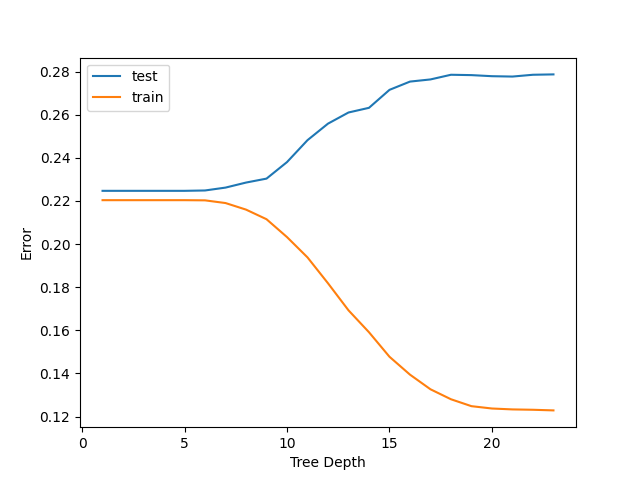
\includegraphics[width=12cm]{q3_decision_tree_plot.png}
    \caption{Decision tree performance on credit default data for q3.}
    \label{fig:q4a}
\end{figure}

\begin{figure}[htp]
    \centering
    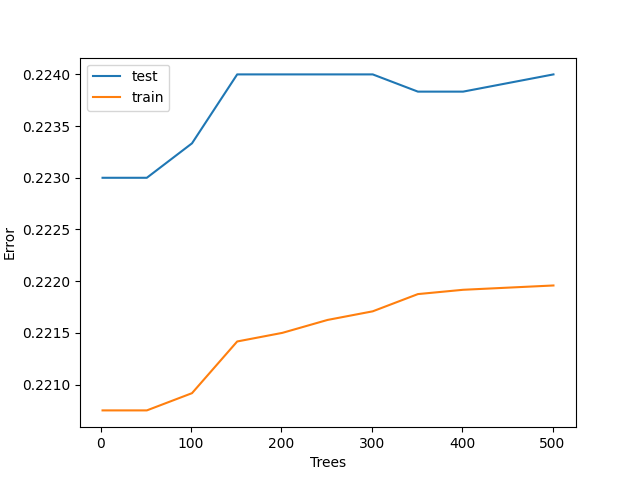
\includegraphics[width=12cm]{q3_adaboost_plot.png}
    \caption{Adaboost performance on credit default data for q3.}
    \label{fig:q4a}
\end{figure}

\begin{figure}[htp]
    \centering
    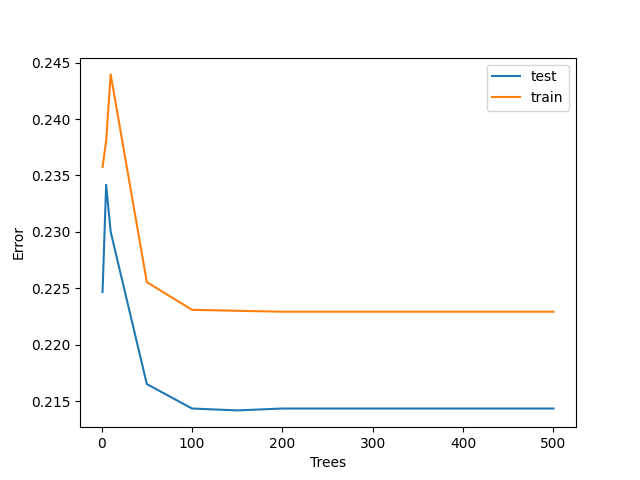
\includegraphics[width=12cm]{q3_bagger_plot.png}
    \caption{Bagger performance on credit default data for q3.}
    \label{fig:q4a}
\end{figure}

\begin{figure}[htp]
    \centering
    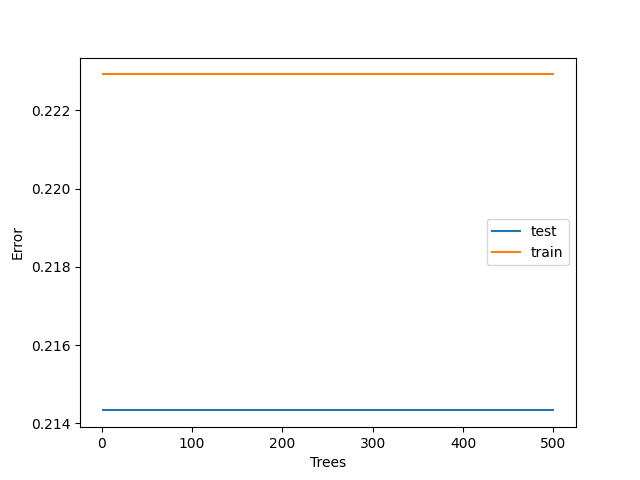
\includegraphics[width=12cm]{q3_random_forest_plot.png}
    \caption{Random forest performance on credit default data for q3.}
    \label{fig:q4a}
\end{figure}

	\item~
	
	\begin{enumerate}
		\item~\emph{Answer}
		
		TEST COST: 41.10059112261912
    
        LEARNING RATE: 0.01
    
        WEIGHT VECTOR
        
        Cement        0.900225
        
        Slag          0.785943
        
        FlyAsh        0.850665
        
        Water         1.298623
        
        SP            0.129834
        
        CoarseAggr    1.571793
        
        FineAggr      0.998347
        
        MODEL\_BIAS   -0.015204
        
        Figure 9 shows how the norm of the difference in weights converge with increasing rounds, while Figure 10 shows how cost converges with increasing rounds.
        
        \begin{figure}[htp]
            \centering
            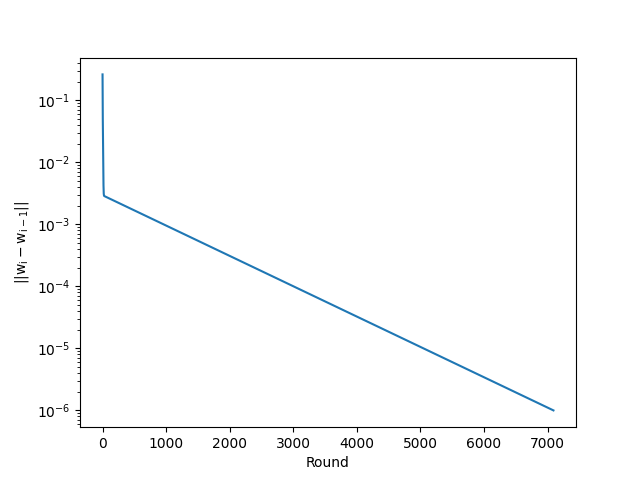
\includegraphics[width=12cm]{part2_q4a_convergence.png}
            \caption{Weight convergence with increasing rounds for q4a.}
            \label{fig:q4a}
        \end{figure}
        
        \begin{figure}[htp]
            \centering
            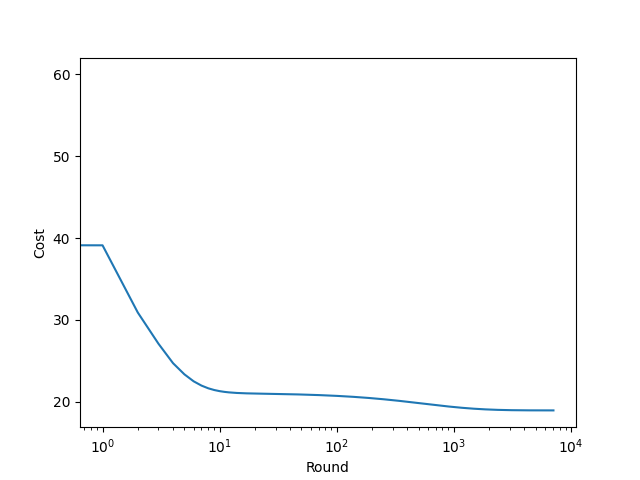
\includegraphics[width=12cm]{part2_q4a_cost.png}
            \caption{Cost convergence with increasing rounds for q4a.}
            \label{fig:q4a}
        \end{figure}
		
		\item~\emph{Answer}
		
		TEST COST: 39.57331988956421
		
		LEARNING RATE: 0.005
        
        WEIGHT VECTOR
        
        Cement        0.036170
        
        Slag         -0.156407
        
        FlyAsh       -0.105242
        
        Water         0.469587
        
        SP           -0.049837
        
        CoarseAggr    0.327384
        
        FineAggr      0.057579
        
        MODEL\_BIAS   -0.0160697
        
        Figure 11 shows how the norm of the difference in weights behave over time, while Figure 12 shows how cost converges with increasing rounds.
        
         \begin{figure}[htp]
            \centering
            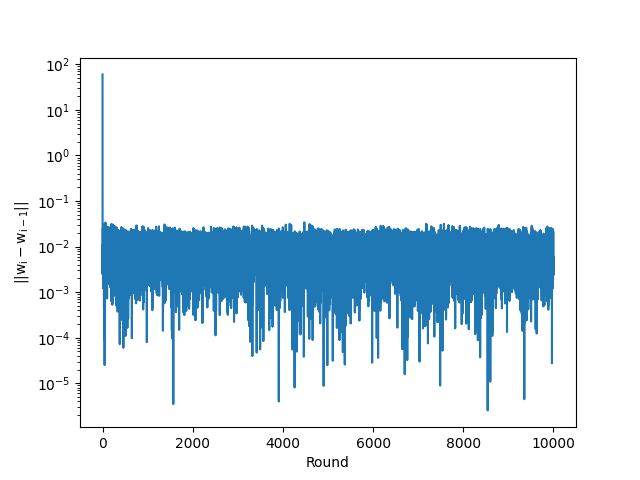
\includegraphics[width=12cm]{part2_q4b_convergence.png}
            \caption{Weight convergence with increasing rounds for q4b.}
            \label{fig:q4a}
        \end{figure}
        
        \begin{figure}[htp]
            \centering
            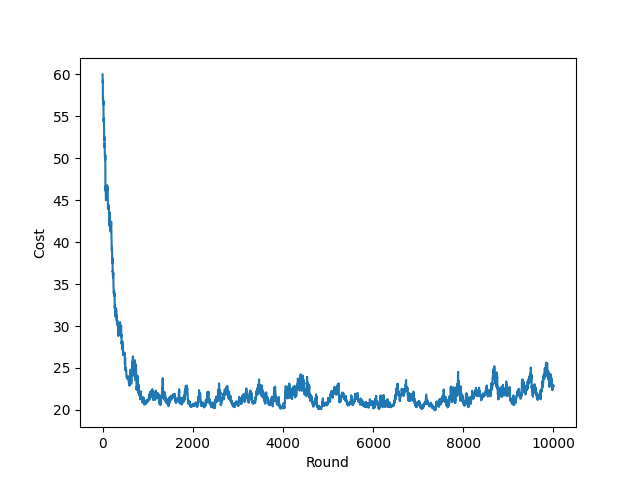
\includegraphics[width=12cm]{part2_q4b_cost.png}
            \caption{Cost convergence with increasing rounds for q4b.}
            \label{fig:q4a}
        \end{figure}
		
		\item~\emph{Answer}
		
		Used the code in Listing 2 to calculate the optimal weights from the input X and y.
		
		\begin{lstlisting}[language=Python, caption=Optimal Weights Function]

def calc_optimal_weights(X: pd.DataFrame, y: pd.Series
        ) -> pd.Series:
    X['MODEL_BIAS'] = 1
    nX = X.to_numpy().T # Has to be transposed 
                        # for lin. alg. to work
    ny = y.to_numpy()
    x_xt = np.matmul(nX, np.transpose(nX))
    x_xt_inv = np.linalg.inv(x_xt)
    x_xt_inv_x = np.matmul(x_xt_inv, nX)
    x_xt_inv_x_y = np.dot(x_xt_inv_x, ny)
    return pd.Series(
        x_xt_inv_x_y, index=X.columns
    )

	    \end{lstlisting}
		
		WEIGHT VECTOR
		
	    Cement        0.900565
	    
        Slag          0.786293
        
        FlyAsh        0.851043
        
        Water         1.298894
        
        SP            0.129891
        
        CoarseAggr    1.572249
        
        FineAggr      0.998694
        
        MODEL\_BIAS   -0.015197
    
        This weight vector corresponds almost exactly to what we observe from Batch Gradient Descent, but is almost entirely different from the results for Stochastic Gradient Descent except for the Bias. Although the costs were about the same for Batch Gradient Descent and Stochastic Gradient Descent (both ~40), their weight vectors ended up being very different. I have two guesses as to what may have happened. One, the SGD algorithm hits a local minimum. Based on multiple runs, I think this may be possible as SGD does not always converge for me, indicating there may likely be a bug, as I get bad results no matter what parameters I plug into SGD. The other guess I have is based on the very similar costs for SGD and BGD. It may be possible that the bias is the most important term here, since that term alone is essentially the same for all three sets of results (~-0.015), and perhaps the weights are simply "close enough" in both BGD and SGD. One test I think that may be interesting to check would be to use both of these models as linear classifiers, and see how their error rates compare. If the error rates are significantly different, then I would conclude that, yes, my SGD algorithm is simply broken and needs to be fixed. I tend to think that this is the most likely case, and will proceed from here with the assumption that I failed to properly implement SGD.
    
	\end{enumerate}

\end{enumerate}

\end{document}
%%% Local Variables:
%%% mode: latex
%%% TeX-master: t
%%% End:
